\documentclass[conf]{new-aiaa}
%\documentclass[journal]{new-aiaa} for journal papers
\usepackage[utf8]{inputenc}

\usepackage{graphicx}
\usepackage{amsmath}
\usepackage[version=4]{mhchem}
\usepackage{siunitx}
\usepackage{longtable,tabularx}
\usepackage[utf8]{inputenc}
\usepackage{titlesec}
\usepackage{indentfirst}
\usepackage{graphicx}
\usepackage{multirow}
\usepackage[table,xcdraw]{xcolor}
\usepackage{longtable}
\usepackage{amsmath}
\usepackage{geometry}
\usepackage[english]{babel}
% \usepackage[backend=biber,style=numeric,citestyle=numeric-comp ]{biblatex}

\setlength\LTleft{0pt}

\title{Multidisciplinary Design Optimization on Maximizing Long-Term Profit for an eVTOL Aircraft}

\author{Jake E Egana}
\author{Abhinav Pradhan}
\author{Marius Ruh}
\author{Zachary Steffish}

\affil{In fulfillment of the requirements for MAE155B}
\affil{University of California, San Diego}
\affil{Department of Mechanical and Aerospace Engineering}

% \addbibresource{references.bib}

\begin{document}


\maketitle

\begin{abstract}
This is an EXAMPLE abstract.
\end{abstract}

\section{Nomenclature}

{\renewcommand\arraystretch{1.0}
\noindent\begin{longtable*}{@{}l @{\quad=\quad} l@{}}
$\alpha$  & angle of attack \\
$AR$ & aspect ratio\\
$S$& area \\
$h$ & altitude \\
$V_\infty$ & airspeed \\
$Q_n$   & normalized torque \\
$R$ & rotor radius \\
$RPM$ & $X$ rotational speed in revolutions per minute \\
$m_b$ & $Y$ battery mass \\
$num. flts$   & number of flights \\
$L$  & lift \\
$W$  & weight \\
$T$  & thrust \\
$D$  & drag \\
$E_{avail}$ & energy available\\
$E_{total}$ & energy total \\
$C_m$ & pitching moment \\
$C_r$ & rolling moment \\
$SM$ & static margin \\
$x$ & distance from nose
\end{longtable*}}

\section{Introduction}

\section{Background}

\section{Methodology}

\pagebreak
\subsection{Problem Statement}
\begin{table}[!hbt]
    \centering
    \caption{Optimization Problem Statement.}
    \begin{tabular}{r l l c c}
        \hline
        & Variable & Description & Quantity\\
        &&& (primary)\\
        \hline
        minimize
        & -Profit \\
        \hline
        with respect to
        & $-3 \le \alpha_{wing} \le 5^{\circ}$ & Wing Angle of Attack & 1\\
        & $3 \le AR_{wing} \le 13$ & Wing Aspect Ratio & 1\\
        & $15 \le S_{wing} \le 30\hspace{1mm}m^{2}$ & Wing Area & 1\\
        & $-3 \le \alpha_{tail} \le 5^{\circ}$ & Tail Angle of Attack & 1 \\
        & $3 \le AR_{tail} \le 13$ & Tail Aspect Ratio & 1 \\
        & $2 \le S_{tail} \le 4\hspace{1mm}m^{2}$ & Tail Area & 1 \\
        & $2 \le x_{tail,c/4} \le 8$ & Location of Tail c/4 & 1 \\
        & $0 \le h \le 2\hspace{1mm}km$ & Altitude & 1 \\
        & $58 \le V_{\infty} \le 70\hspace{1mm}m/s$ & Speed & 1 \\
        & $0 \leq Q_n \leq 0.6$ & Normalized torque & 6 \\
        & $100 \leq Range \leq 300 km$ & Range & 1 \\
        & $* \le R \le *$ & Rotor Radius & 3 \\
        & $1900 \le RPM \le 3000$ & Rotational Speed in RPM & 6 \\
        & $500 \le m_{b} \le 700\hspace{1mm}kg$ & Battery Mass & 1 \\
        & $0 \le num.\hspace{1mm}flts. \le 200$ & Number of Flights & 1 \\
        \cline{3-5}
        && Total design variables & 27 \\
        \hline
        subject to
        & $L-W=0$ & Vertical Equilibrium & 1 \\
        & $T-D=0$ & Horizontal Equilibrium & 1 \\
        & $E_{total} \le 10E_{avail}$ & Energy Constraint & 1\\
        & $C_{m}=0$ & Pitching Moment  & 1 \\
        & $C_{r}=0$ & Rolling Moment & 1 \\
        & $6\% \leq SM \leq 20\%$ & Static Margin & 1 \\
        \cline{3-5}
        && Total constraints & 6 & \\
        \hline
    \end{tabular}
    \label{tab:optprob}
\end{table}
\pagebreak

\pagebreak
\subsection{Design Structure Matrix}
The design structure matrix is shown in figure [citation]. It visualizes the design optimization problem.
\begin{figure}[!hbt]
    \centering
    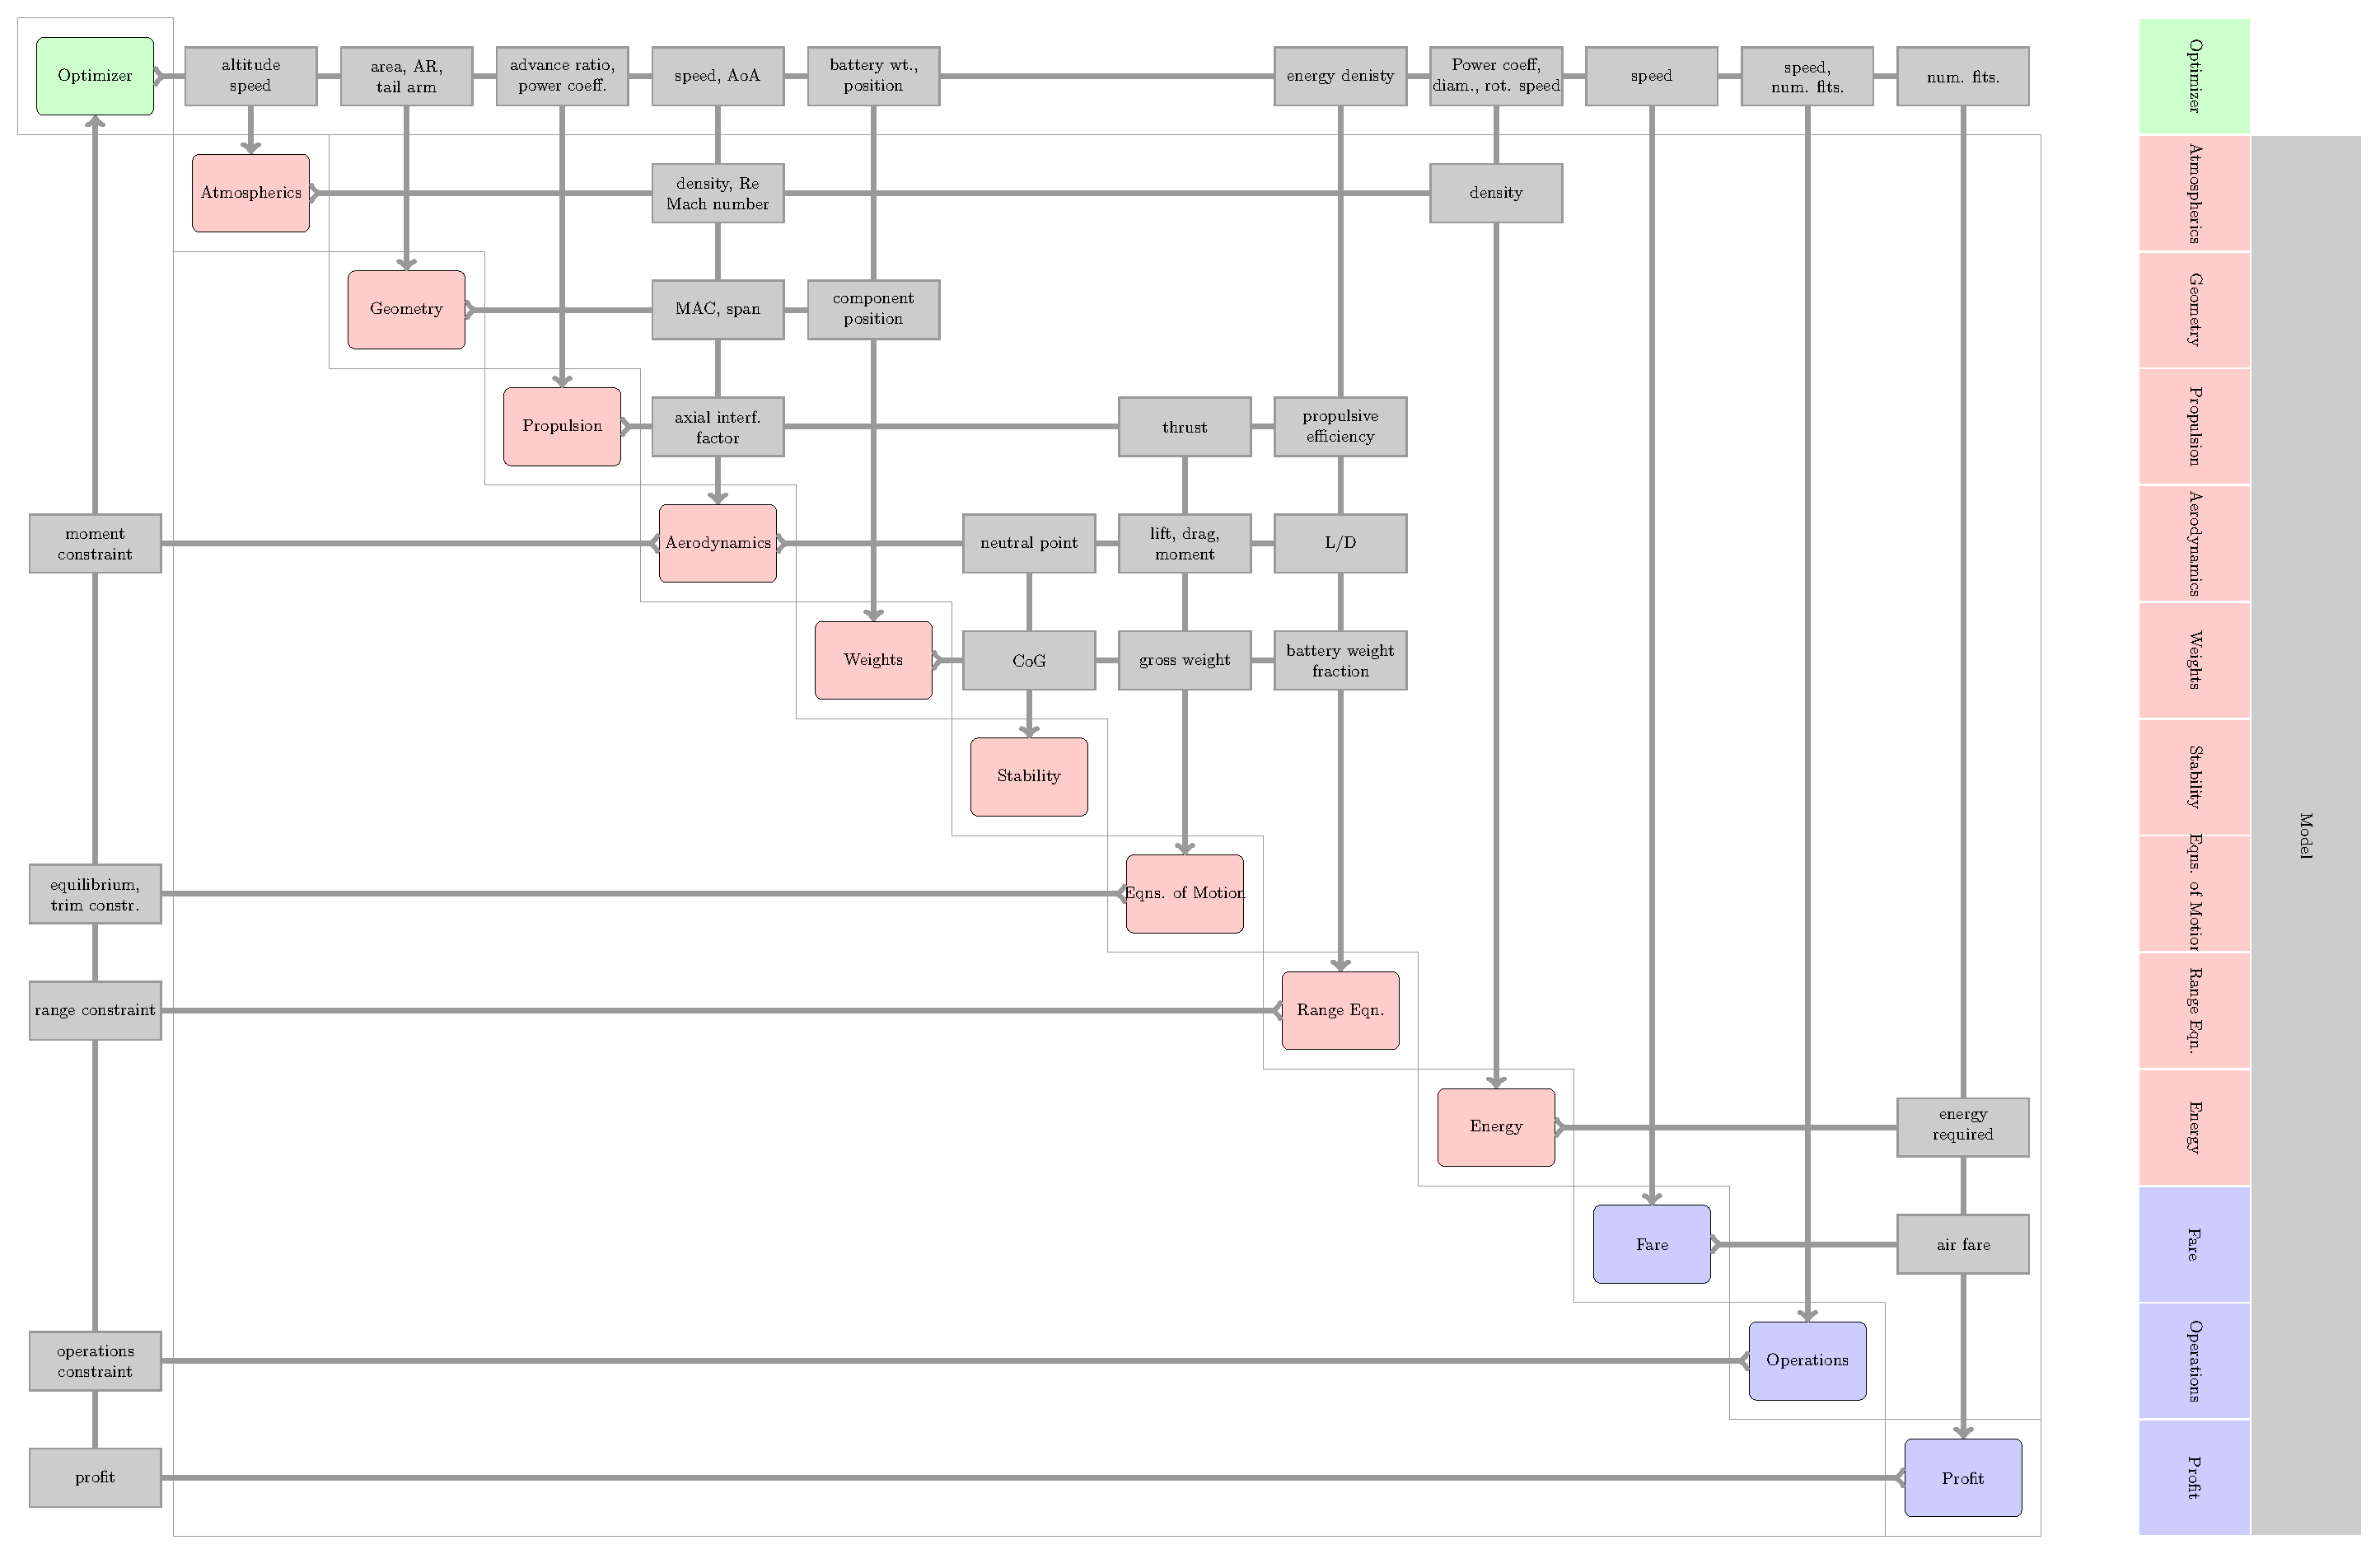
\includegraphics[angle=90, height=20cm] {images/a_2_dsm.pdf}
    \caption{Design Structure Matrix (DSM) for Optimization problem}
    \label{fig:my_label}
\end{figure}
\pagebreak

\subsection{Software Description}

\section{Models}

\subsection{Aerodynamics}
The aerodynamic model is based on empirical formulae used to calculate lift and drag. To determine the lift and drag coefficient, standard 2-D airfoil analysis is employed that assumes linearity in the lift coefficient. In addition, in order to account for the section of the wing that is affected by the increased velocity of the slipstream due to the propellers,~\cite{first} includes a slightly modified formulation for the lift coefficient, which is shown in equation (1).
\begin{equation}\label{modified_Cl}
C_{L} = C_{L_{0}} + \frac{2r(C_{L_{0}}(1+aC_{b})^{2}-C_{L_{0}})*blown\: percentage}{span}
\end{equation}
where r is the radius, a is the axial induction factor, and C\textsubscript{b} is the blown coefficient factor. This model includes a simplified approach to include the effect of the axial induced velocity, resulting from the propeller slip stream. Including this effect in our analysis was deemed reasonable since we have multiple propellers along the wing with relatively large diameter. \cite{inproceedings_2} models this effect more thoroughly, however, we decided that for our purposes a lower fidelity aerodynamic model suffices as our objective function is profit and therefore less emphasis is placed on the design. The induced drag is calculated in the standard manner from the lift coefficient and by assuming a reasonable value for the Oswald efficiency factor. Also, the skin friction and form drag is estimated using the drag build up equations. The vortex lattice method (VLM) was also considered as it is a high-fidelity method that allows for accurate modelling of the aerodynamics as well as the effects of the slipstream. However, we decided that this level of fidelity was not necessary.

\subsection{Propulsion}
The propulsion model relies on the Glauert propeller theory, which is a high-fidelity model derived from general momentum theory. One of the main advantages of the Glauert model is that it includes the various losses associated with propeller motion. Since our aircraft is propeller driven, it was deemed appropriate to employ a high-fidelity propulsion model. The Glauert model is summarized by the following set of equations taken from \cite{israel}:
 \begin{equation}\label{modified_Cl}
 \begin{gathered}
\eta = \eta_{1}\eta_{2}\eta_{3},\:\eta_{2} = 1 - \frac{4\eta_{1}}{\pi^{3}J}C_{P},\:\tan\varphi_{1} =\frac{J}{\pi\eta_{1}\eta_{2}} \\ \eta_{3} = 1 - \frac{\pi^{4}}{8}\frac{\eta_{2}^{2}}{C_{P}}\sigma\bar{C_{d}}f(\varphi_{1}), \: \eta_{1} = 1 - \frac{2}{\pi}C_{P}\eta_{2}\eta_{3}\left(\frac{\eta_{1}}{J}\right)^{2}
   \end{gathered}
\end{equation}
where $\eta_{1}$, $\eta_{2}$, $\eta_{3}$ are the efficiencies associated with the losses due to the axial induced velocity, the rotational velocity and blade drag of the propeller, respectively. In addition, J is the advance ratio and $C_{P}$ is the power coefficient. Lastly, $\sigma$,$\bar{C_{d}}$ and $\varphi_{1}$ are the blade solidity, the blade-average two-dimensional (2-D) drag and the the inflow angle between the propeller disk plane and the resultant cross-sectional velocity. Once the overall propulsive efficiency is determined it is easy to compute the thrust coefficient ($C_{T}$) and ultimately the thrust (T), which are related to the efficiency by the subsequent pair of equations:
 \begin{equation}\label{modified_Cl}
 \begin{gathered}
\eta = \frac{C_{T}J}{C_{P}},\:C_{T}=\frac{T}{\rho n^{2}D^{4}}
   \end{gathered}
\end{equation}
where $\rho$ is the density and D is the blade diameter. While the Glauert model presented above accurately accounts for the losses associated with the blade motion, it assumes that the losses are solely due the aerodynamic action of the propeller. In reality, however, there is an additional loss resulting from the interaction between the air and the so called propeller boss \cite{aero}. Unfortunately, there is no literature yet available that includes this effect in the Glauert model.

\subsection{Performance}
In this optimization problem we are only considering the cruise segment of the mission profile and therefore the net force acting on the aircraft has to be equal to zero to achieve steady level flight conditions. For vertical equilibrium, this means that the gross weight equals the lift generated from the wing and tail. It is important that the pitching moment generated from the separate lifting surfaces is equal to zero. To guarantee horizontal equilibrium, the cruise condition implies that the forward thrust generated from the propeller equals the parasitic and induced drag. The main reason that only the cruise condition is considered is that range is one of the constraints and the range equation for electric aircraft is only valid for steady level flight.

\subsection{Weights and Stability}
The model utilized for weights and stability is comprised of the equations outlined by Raymer's design reference \cite{raymer}. Namely, the equations for general aviation were used to obtain output values for the aircraft's empty weight, center-of-gravity location, and neutral point location. This model was selected for the reason that it provides a high level of flexibility without sacrificing simplicity; moreover, it is based on Raymer’s empirical estimations and so provides us with a way to consider the feasibility of each weight estimate. Raymer’s equations for weight-by-component were subsequently utilized to provide estimates for the aircraft’s center-of-gravity (CG) and neutral point (NP), as outlined in equations (4) and (5).

\subsection{Economics}
The economics model is based on several formulae, including the Development and procurement costs of aircraft (DAPCA) equations and modifying them for an eVTOL aircraft. The main inputs are empty aircraft weight, maximum velocity, and the quantity of aircraft to be produced. The model outputs a total cost for the research, development, testing, and evaluation of the aircraft. To find labor costs for manufacturing, tooling, engineering and quality control, research was conducted to find the average hourly rate for each individual specialty. The engine production cost equation was removed and replaced with a battery and motor cost analysis, using a modern day value for cost per kilowatt-hr for the battery, and a standard market value for the motors.

\subsection{Approach}

\section{Conclusion}

\subsection{Summary}

\subsection{Significance}

\subsection{Future}

\section{Individual Contributions}

% \section*{Appendix}

\bibliographystyle{plain}
\bibliography{references.bib}

\end{document}
